\section{Mass hierarchy sensitivity}
\label{sec:mh_sens}

\begin{figure}[htbp]
  \centering
  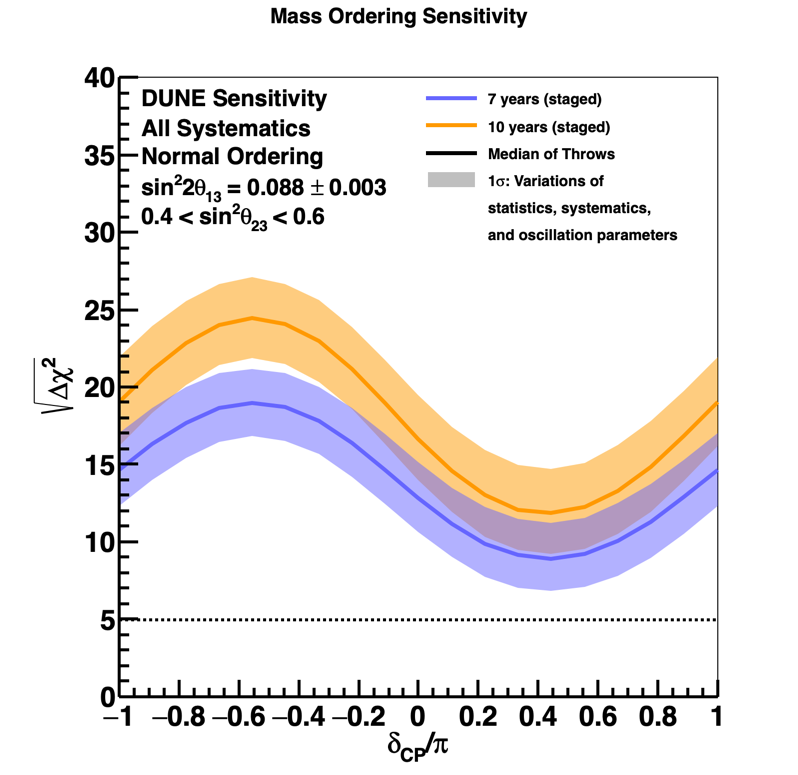
\includegraphics[width=0.98\linewidth, trim={0cm 0cm 0cm 2.3cm}, clip]{mh_two_exps_throws_nh_2019_v4.png}
  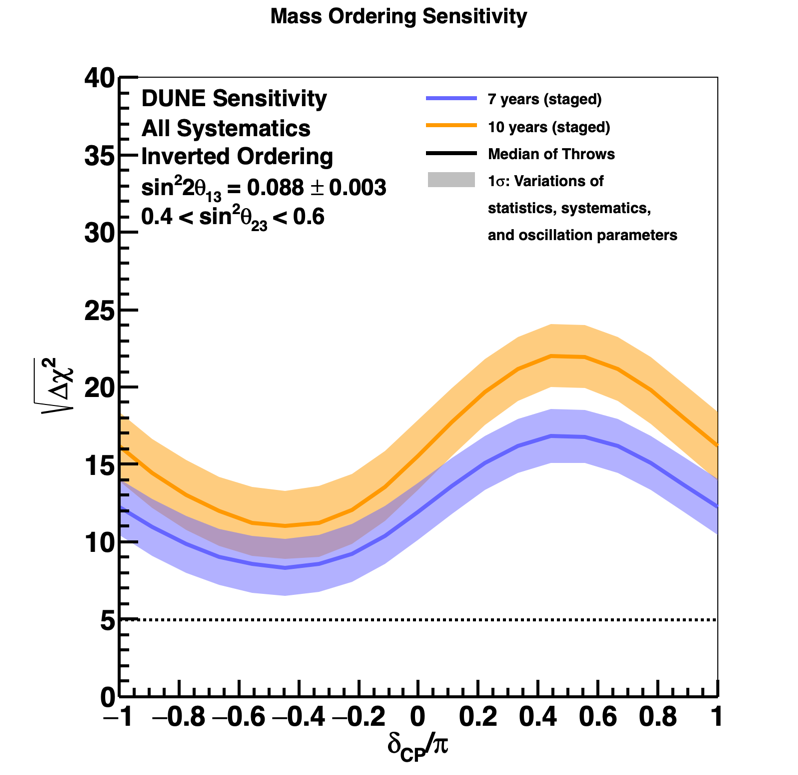
\includegraphics[width=0.98\linewidth, trim={0cm 0cm 0cm 2.3cm}, clip]{mh_two_exps_throws_ih_2019_v4.png}
  \caption[Significance of the DUNE neutrino mass ordering determination, as a function of \deltacp]{Significance of the DUNE determination of the neutrino mass ordering, as a function of the true value of \deltacp, for seven (blue) and ten (orange) years of exposure. The width of the transparent bands cover 68\% of fits in which random throws are used to simulate statistical variations and select true values of the oscillation and systematic uncertainty parameters, constrained by pre-fit uncertainties. The solid lines show the median sensitivity.}
  \label{fig:mh_nominal}
\end{figure}
Figure~\ref{fig:mh_nominal} shows the significance with which the neutrino mass ordering can be determined in both \dword{no} and \dword{io} as a function of the true value of \deltacp, for both seven and ten year exposures, including the effect of all other oscillation and systematic parameters using the toy throwing method described in Section~\ref{sec:methods}. The characteristic shape results from near degeneracy between matter and \dword{cpv} effects that occurs near $\deltacp=\pi/2$ ($-\deltacp=\pi/2$) for true normal (inverted) ordering. Studies have indicated that special attention must be paid to the statistical interpretation of neutrino mass ordering sensitivities~\cite{Ciuffoli:2013rza,Qian:2012zn,Blennow:2013oma} because the $\Delta\chi^2$ metric does not follow the expected chi-square function for one degree of freedom, so the interpretation of the $\sqrt{\Delta \chi^{2}}$ as the sensitivity is complicated. However, it is clear from Figure~\ref{fig:mh_nominal} that \dword{dune} is able to distinguish the mass ordering for both true \dword{no} and \dword{io}, and using the corrections from, for example, Ref.~\cite{Ciuffoli:2013rza}, DUNE would still achieve 5$\sigma$ significance for the central 68\% of all throws shown in Figure~\ref{fig:mh_nominal}. We note that for both seven and ten years (it was not checked for lower exposures), there were no parameter throws used in generating the plots ($\sim$300,000 each) for which the incorrect mass ordering was preferred.

\begin{figure*}[htbp]
  \centering
  \subfloat[6 ktMWyr]   {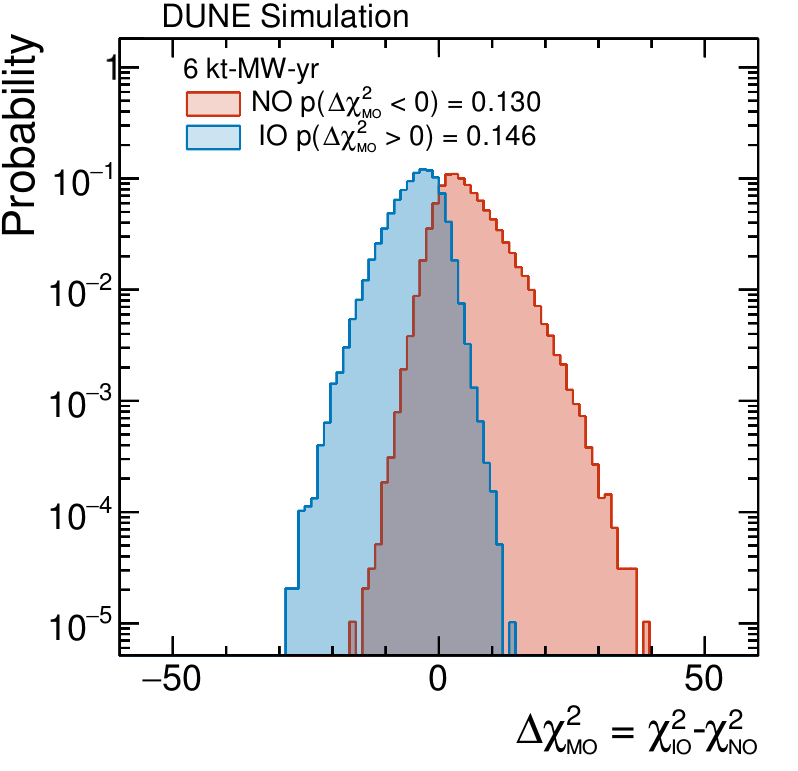
\includegraphics[width=0.33\linewidth]{MH_comp_ndfd_6ktMWyr_th13.png}}
  \subfloat[12 ktMWyr]  {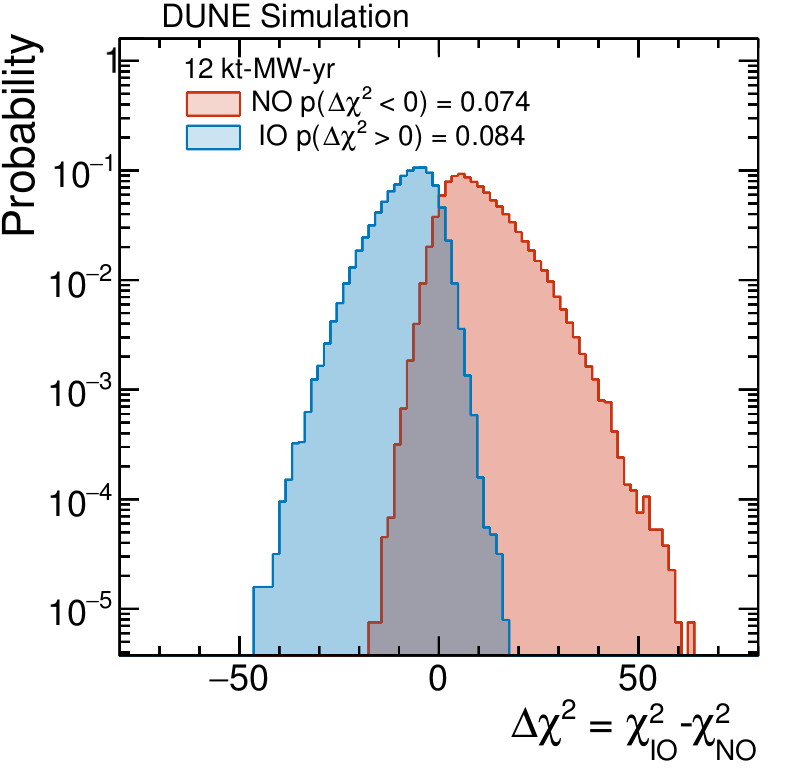
\includegraphics[width=0.33\linewidth]{MH_comp_ndfd_12ktMWyr_th13.png}}
  \subfloat[24 ktMWyr]  {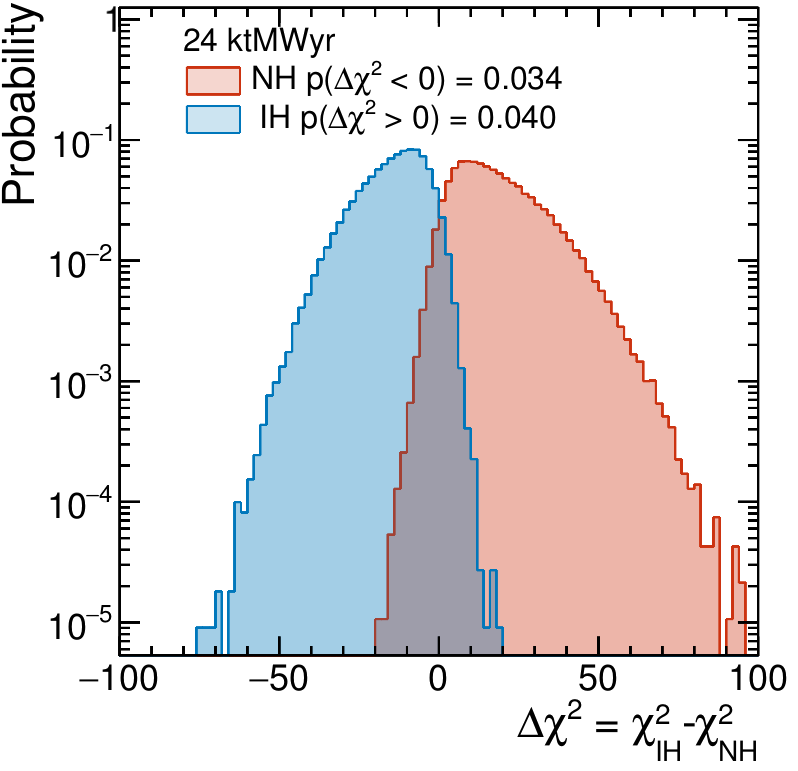
\includegraphics[width=0.33\linewidth]{MH_comp_ndfd_24ktMWyr_th13.png}}\\
  \subfloat[66 ktMWyr]  {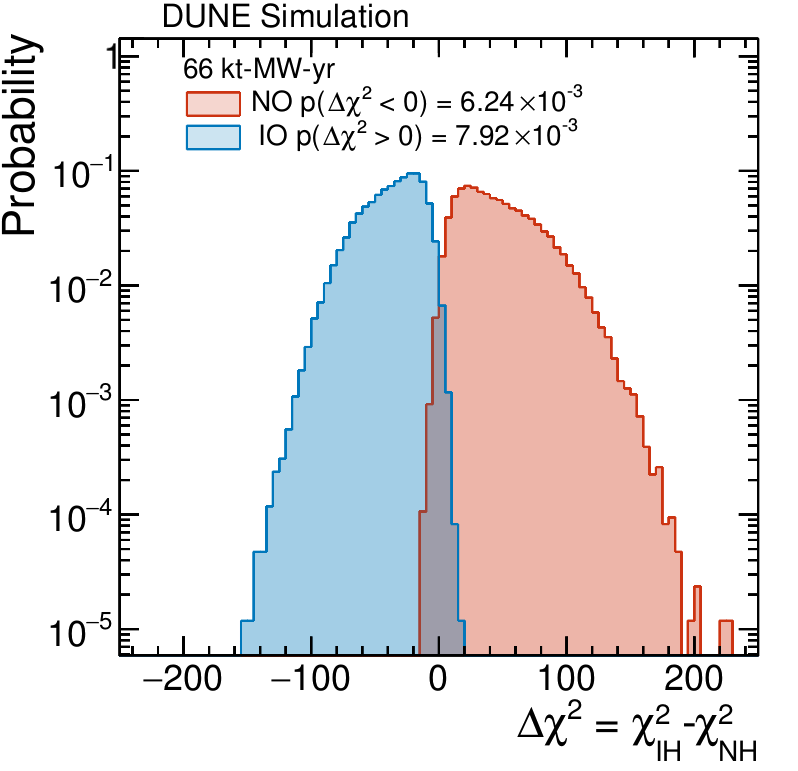
\includegraphics[width=0.33\linewidth]{MH_comp_ndfd_66ktMWyr_th13.png}}
  \subfloat[100 ktMWyr] {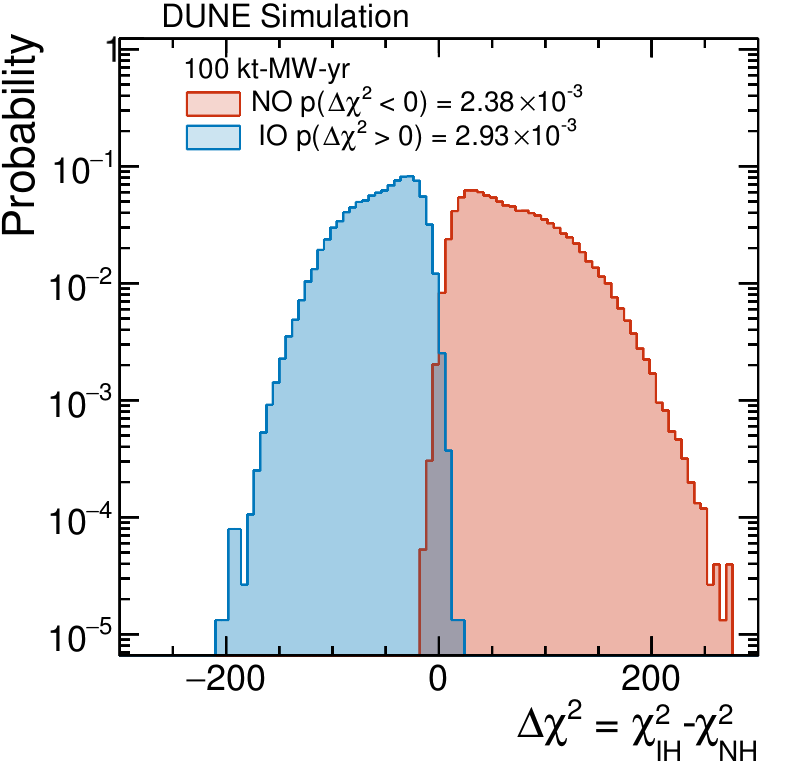
\includegraphics[width=0.33\linewidth]{MH_comp_ndfd_100ktMWyr_th13.png}}
  \subfloat[336 ktMWyr] {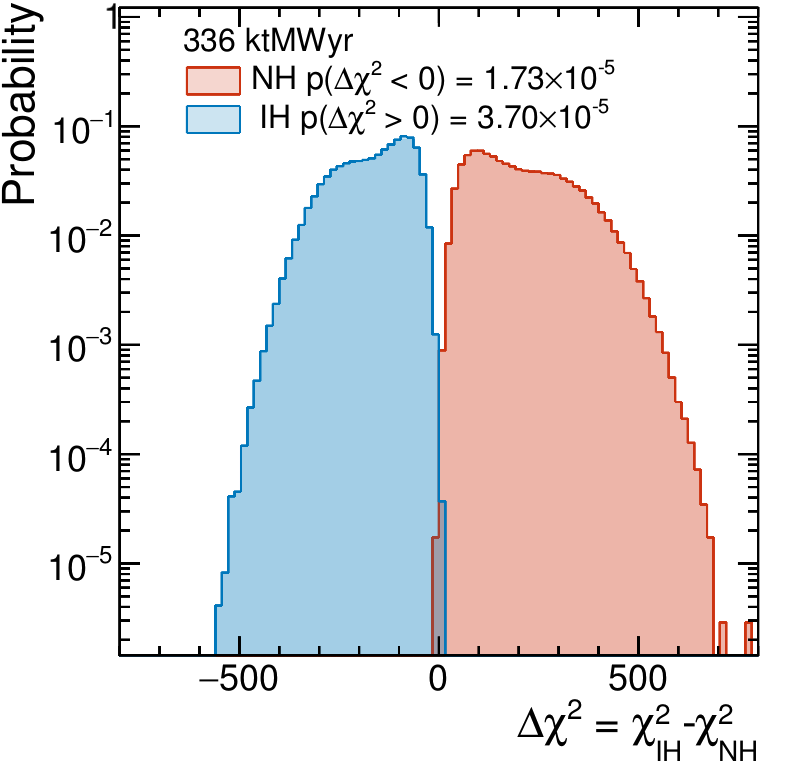
\includegraphics[width=0.33\linewidth]{MH_comp_ndfd_336ktMWyr_th13.png}}
  \caption[]{}
  \label{fig:mh_comp_over_time}
\end{figure*}

\begin{figure*}[htbp]
  \centering
  \subfloat[6 ktMWyr]   {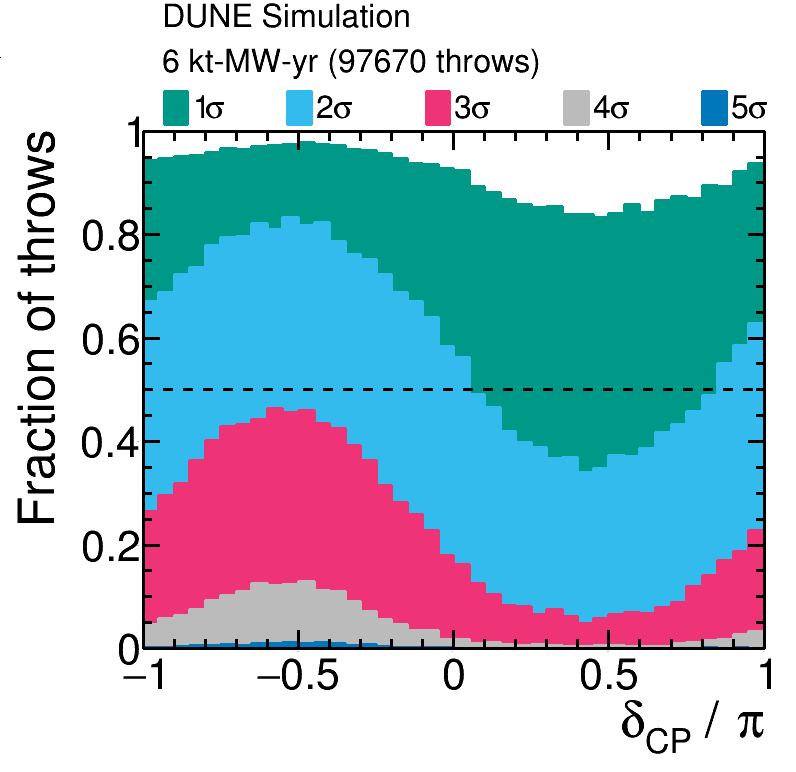
\includegraphics[width=0.33\linewidth]{mh_throws_6ktMWyr_NH_th13.png}}
  \subfloat[12 ktMWyr]  {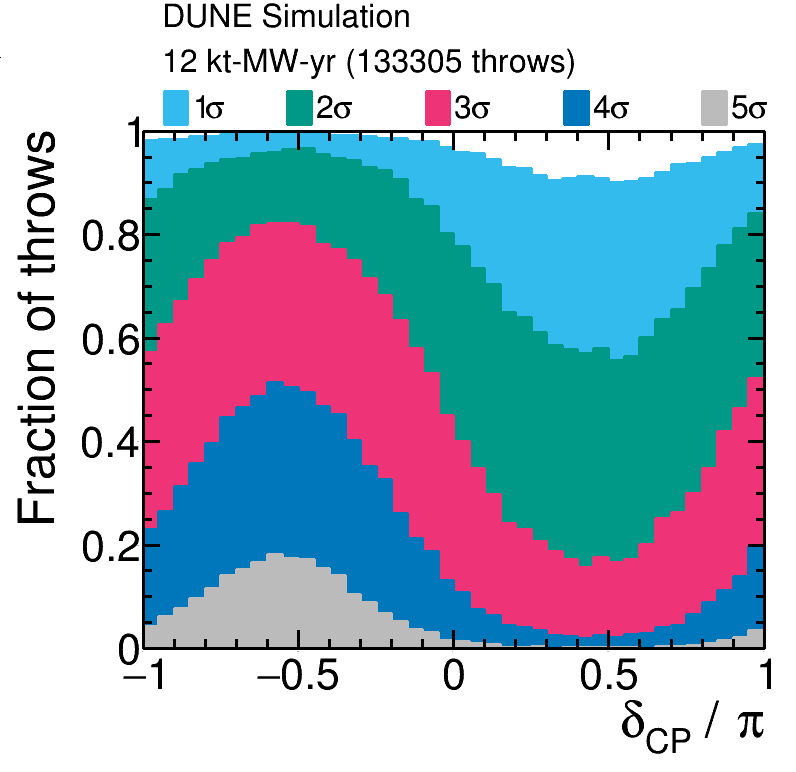
\includegraphics[width=0.33\linewidth]{mh_throws_12ktMWyr_NH_th13.png}}
  \subfloat[24 ktMWyr]  {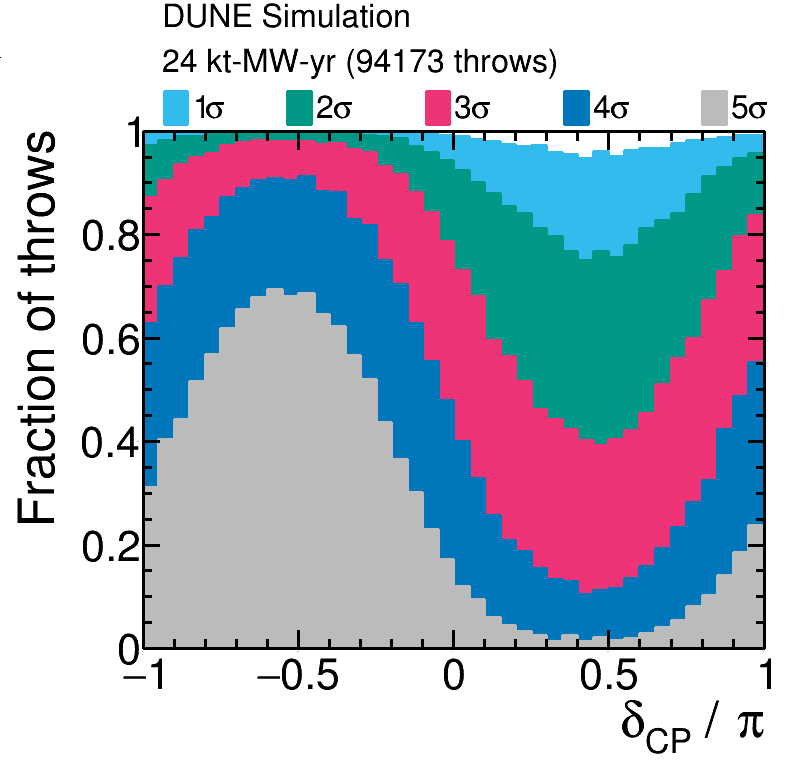
\includegraphics[width=0.33\linewidth]{mh_throws_24ktMWyr_NH_th13.png}}\\
  \subfloat[66 ktMWyr]  {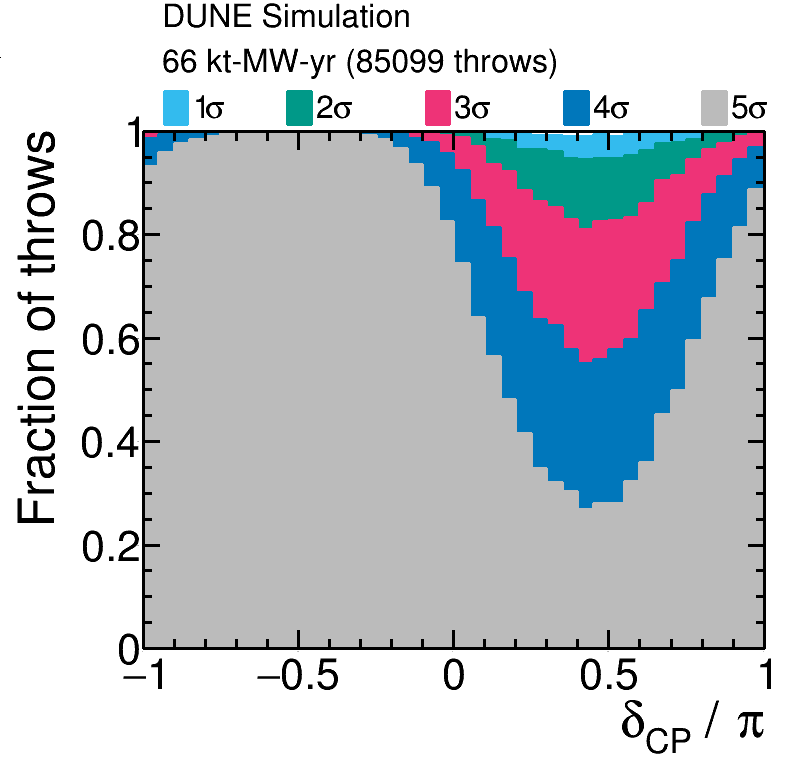
\includegraphics[width=0.33\linewidth]{mh_throws_66ktMWyr_NH_th13.png}}
  \subfloat[100 ktMWyr] {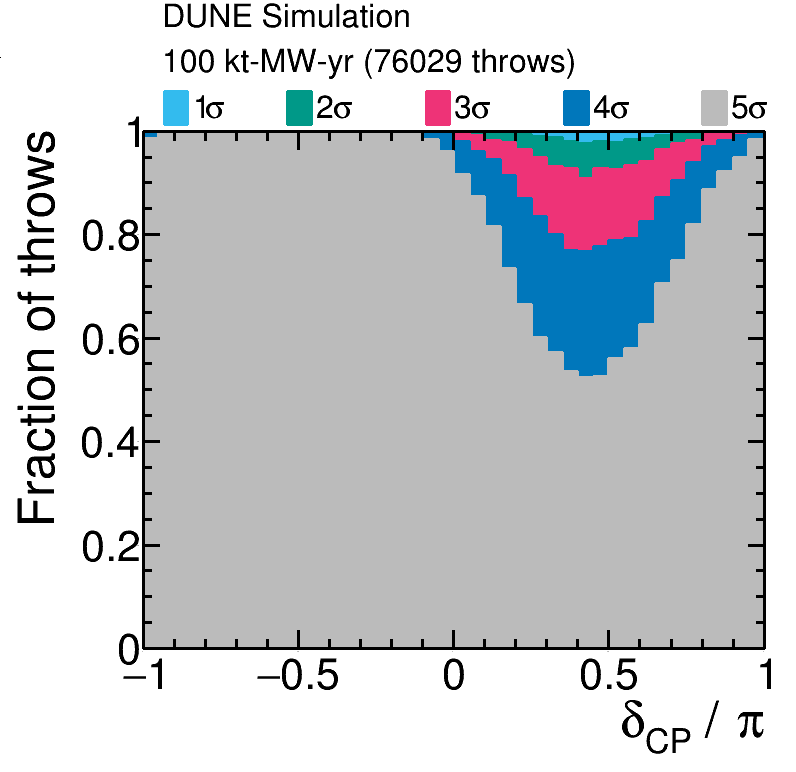
\includegraphics[width=0.33\linewidth]{mh_throws_100ktMWyr_NH_th13.png}}
  \subfloat[336 ktMWyr] {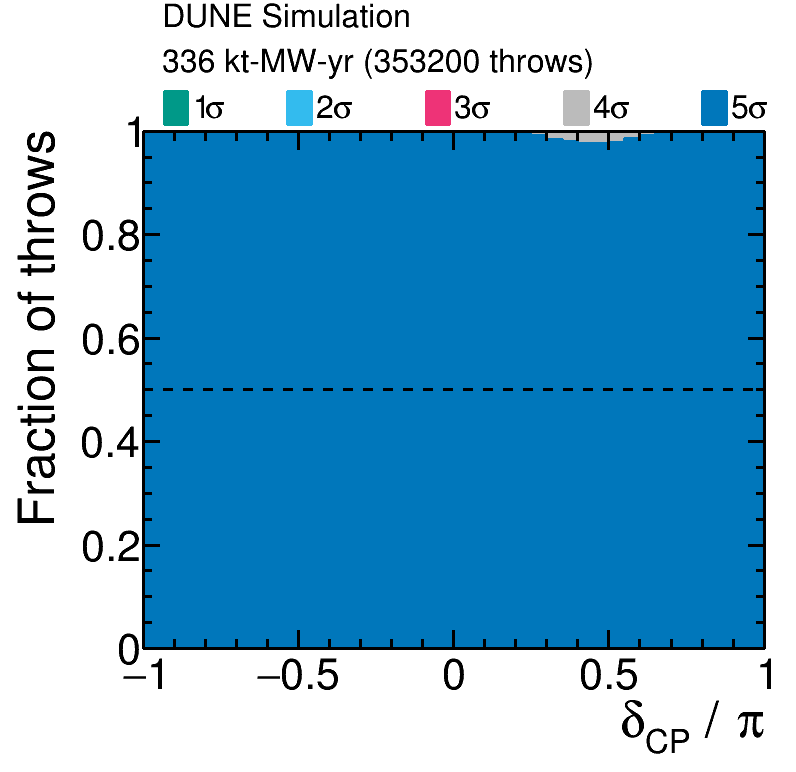
\includegraphics[width=0.33\linewidth]{mh_throws_336ktMWyr_NH_th13.png}}
  \caption[]{}
  \label{fig:mh_nh_over_time}
\end{figure*}
